% Copyright (c) Chris Paxton 2026
% Licensed under the Apache License, Version 2.0.
\section{Agent architecture, tools, and evidence boundaries}
\label{app:combined_agent}

\paragraph{Two orchestrators share interfaces.}
The scored \texttt{EQA\_EPISODE} loop and interactive \texttt{CHAT} loop are distinct.
EQA uses \texttt{AgenticEQAExecutor}: the historical router-off condition selects
from recalled evidence with a deterministic policy, while router-on uses a
language model. Both call the EQA skills described in
Appendix~\ref{app:agentic_tools} and terminate with an answer or exploration budget.
CHAT uses \texttt{run\_agent\_with\_robot} through \texttt{emet run agent}; a language
model selects public tools from a context-bound registry, reads their outcomes,
and chooses its next call. Terminal and Discord share this CHAT loop.
\texttt{--eqa} enables caption support; \texttt{--eqa-eval} delegates to the scored
Habitat episode runner rather than evaluating the CHAT policy. Shared perception,
memory and skill interfaces do not make these controllers interchangeable.

\begin{table}[ht]
\centering
\small
\begin{tabular}{@{}p{.20\linewidth}p{.75\linewidth}@{}}
\toprule
CHAT capability & Representative tools and admission \\
\midrule
Observation and memory & \texttt{describe\_scene}, \texttt{send\_image},
\texttt{query\_memory}, \texttt{query\_scene\_graph},
\texttt{list\_scene\_relations}; historical retrieval is not fresh execution evidence. \\
Navigation and views & \texttt{explore}, \texttt{find\_objects},
\texttt{scan\_environment}, \texttt{go\_home}, \texttt{rotate\_base},
\texttt{face\_toward}, \texttt{move\_forward}, \texttt{observe\_floor};
robot capabilities, measured arrival and map coverage constrain actions. \\
Primitive TAMP & \texttt{scene\_tasks}, \texttt{plan\_pick\_place},
\texttt{execute\_pick\_place\_plan}, \texttt{pick\_place};
input provenance and execution mode are checked independently. \\
Multi-step TAMP & \texttt{plan\_task}, \texttt{execute\_task\_plan};
exposed only with a bound provider, currently a privileged stationary Stretch
transfer provider for the native diagnostics. \\
Articulation & \texttt{set\_receptacle\_state}; simulator-assisted joint setting,
rejected by native physical execution. \\
\bottomrule
\end{tabular}
\caption{CHAT capability groups. Registration and shared tool names do not
establish successful composition or availability on every robot. Complete public
schemas and mode qualifications are maintained in the repository tool index.}
\label{tab:chat_capabilities}
\end{table}

\paragraph{Language selects goals; planners refine motion.}
A task request passes from CHAT to a grounded task session, then to task-skeleton
search, per-step motion refinement, actuation, and measured-effect verification.
Greedy, beam and UCT use the same operator/feasibility interface. The bounded
instruction compiler accepts explicit move clauses and swaps; it is not an
unrestricted natural-language task compiler. Unmentioned objects' initial
location predicates are protected. A returned skeleton is not a full-episode
collision-free trajectory certificate: later transfers must be replanned from
fresh measured geometry. Ordered lift/orient/extend pregrasp avoids falling back
to a simultaneous arm sweep when the ordered route is blocked.

\paragraph{Structured outcomes govern continuation.}
Versioned JSON reports status, public failure code, recovery instruction and
opaque one-shot handles. Execution rejects changed scene/robot identity and
state, verifies each operator's effects and protected goals, and checks final
goals. A planning-only or provider-preflight failure returns a no-actuation
receipt with \texttt{failed\_phase=preflight}. If earlier steps succeeded, their
completed count and partial progress remain visible. An exception after entering
the executor is conservatively treated as possible actuation. Failed, partial,
malformed, uncertain and discovery-only outcomes stop further dispatch for that
user turn. A new user turn permits inspection/replanning, not silent reuse of a
consumed handle. The task prompt requests one tool call per round; the dispatcher
also enforces stop boundaries within a precomputed batch.

\paragraph{Budget and inference conditions.}
CHAT defaults to three tool rounds and exposes a range of 1--32; the native
controls use 12. A separate no-tool final summary may add a model call. Task
search and native IK probes have bounded work, but the proposed shared
whole-agent ledger is not wired through every model and execution-replanning
call; no matched total-call/cost baseline is claimed. Remote OpenAI-compatible
text and vision clients keep measured robot telemetry live during inference.
The stationary controls use Caliban-hosted Qwen3-VL-8B-Instruct in text/tool mode,
with camera input disabled. They select the DynaMem backend explicitly, whereas
normal interactive CHAT defaults to Dynagraph. Their physics advances
asynchronously during inference; native stepped benchmark horizons are a
separate runtime condition.

\paragraph{Observed integration remains a gate.}
The current RGBD discovery provider estimates visible positions and heuristic
support patches, not complete object pose, volume, contact or stable grasp.
It therefore remains read-only. The observed-integration path retains capture identity through perception and invalidates
evidence/plan handles around CHAT navigation and view motion. Cached capture
publication cannot renew its local evidence age, and in-flight pre-motion
segmentation cannot publish afterward. The live-camera binding reuses bounded
semantic references while obtaining current geometry from the robot's existing
RGBD stream on discovery requests, without another semantic model call. Missing
or ambiguous evidence rejects the update instead of renewing cached geometry.
This refreshes visible positions, not full object pose or executable affordances.
A separately injected experimental native adapter consumes material-landmark RGBD
tracking, declared conservative geometry and temporally bounded visual effects
through the same primitive and task tools. Robot-only integration tests, including
a buffered swap, use synthetic feedback and do not qualify live sensor-driven
execution; the default discovery provider does not instantiate this adapter.
An experimental geometry tracker also fits declared primitive priors or measured
multi-view surfaces, retaining distinct pose candidates and unobservable shape
symmetries. Surface-fit residuals are diagnostics, not calibrated pose-error
bounds. Geometry co-motion checks therefore remain separate from temporally
qualified execution evidence and do not add observed task successes.
An opt-in simulator renderer co-samples images and motor feedback from one private
physics snapshot. A separate full-robot debug channel includes unmeasured passive
joints and is rejected by observed effect admission. Motor-only rigid EE FK does
not establish conservative fingertip geometry or hardware calibration.
An explicit shape-equivalent evidence contract now lets experimental payload,
retention and effect consumers handle declared primitive symmetry without
inventing material yaw; generic unique-pose consumers still reject that evidence.
Its error bounds are supplied independently, not inferred from fit residuals.
Analytic passive-joint intervals condition whole-tool gripper envelopes on the
eight motor channels and model assumptions. Two development contact controls
contain all sampled collision volumes in 175 snapshots, including 75 snapshots
with target contact; this is neither a hardware certificate nor 175 independent
tasks. A moving RGBD association diagnostic passes two rendered translation/lift
views and two explicit ambiguity/loss cases. Those fixtures use operator colour
initialization, a complete cylinder prior and ideal rendered depth, rather than
agent semantic grounding or observed enclosure construction.
In a Stretch contact episode using separate calibrated RGB/depth optical frames
and registered measured depth, tracking accepts 11 captures before stopping on
insufficient geometry near the gripper as target visibility decreases.
The privileged contact controller still completes; observed tracking and task
acceptance remain separate (Figure~\ref{fig:observed_moving_geometry}).
Capture identity/order does not establish
cross-host clock synchronization or certify capture-after-motion. These guards
do not enable observed manipulation or validate the full exploration--navigation--
manipulation chain. Privileged simulator state/contact may support independent
scoring and debugging; it is not a claim that equivalent sensors exist on
hardware. Appendix~\ref{app:native_tamp} keeps these evidence tiers separate.

\begin{figure}[ht]
  \centering
  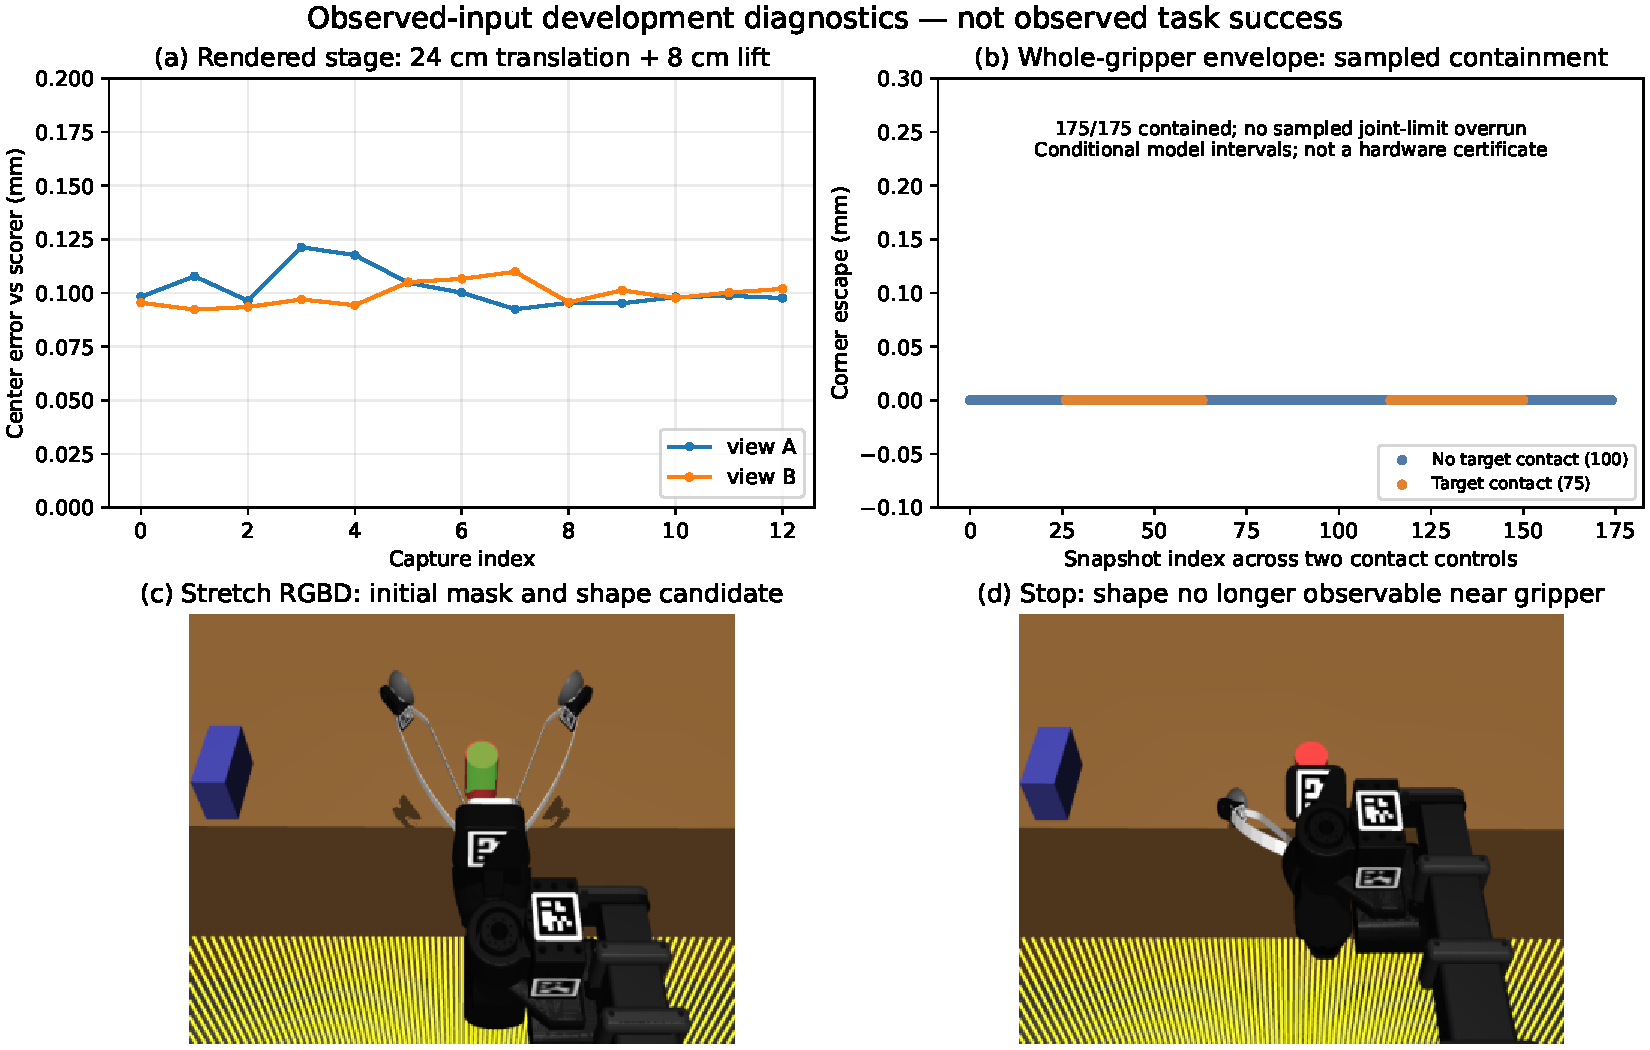
\includegraphics[width=\linewidth]{figures/observed_moving_geometry_20261029.pdf}
  \caption{Observed-input development diagnostics, not observed task success.
  (a) Center error against an independent simulator scorer during 24\,cm stage
  translation and 8\,cm lift, from two views with a declared cylinder prior and
  ideal depth. (b) Conditional whole-gripper model envelopes contain all sampled
  collision-geom corners in two native contact controls; no sampled joint-limit
  overrun occurs. (c--d) Head RGBD initially supports an object candidate, then
  stops near the approaching gripper. Visible target pixels fall from 1349 to
  513 at loss. Simulator segmentation/poses/contacts are evaluator inputs only;
  the demonstrated controller is privileged, and tracking loss remains latched.
  Full observed source assembly, informative contact views and hardware error
  qualification remain unvalidated.}
  \label{fig:observed_moving_geometry}
\end{figure}
